\documentclass[answers]{exam}
\usepackage[utf8]{inputenc}
\usepackage{amsmath}
\usepackage{titling}
\usepackage{float}
\usepackage{csvsimple}

\usepackage{graphicx}
\graphicspath{ {/} }

\setlength{\parindent}{0em}
\setlength{\parskip}{0.5em}

\newcommand{\oneline}{\fillwithlines{0.25in}}
\newcommand\tab[1][1cm]{\hspace*{#1}}

\newcommand{\duedate}{March 4, 2018}
\date{\duedate}

\usepackage{listings}
\usepackage{color}

\definecolor{dkgreen}{rgb}{0,0.6,0}
\definecolor{gray}{rgb}{0.5,0.5,0.5}
\definecolor{mauve}{rgb}{0.58,0,0.82}

\lstset{frame=tb,
  language=C,
  aboveskip=3mm,
  belowskip=3mm,
  showstringspaces=false,
  columns=flexible,
  basicstyle={\small\ttfamily},
  numbers=none,
  numberstyle=\tiny\color{gray},
  keywordstyle=\color{blue},
  commentstyle=\color{dkgreen},
  stringstyle=\color{mauve},
  breaklines=true,
  breakatwhitespace=true,
  tabsize=3
}

\def\therefore{\boldsymbol{\text{ }
\leavevmode
\lower0.4ex\hbox{$\cdot$}
\kern-.5em\raise0.7ex\hbox{$\cdot$}
\kern-0.55em\lower0.4ex\hbox{$\cdot$}
\thinspace\text{ }}}

\pagestyle{headandfoot}
\headrule
\header{Project 1 Report}{Joseph A. Boyle}{\duedate}

\title{Project 1 Report}
\author{Joseph A. Boyle}

\begin{filecontents*}{b_times.csv}
file, fiveregs, tenregs, twentyregs
report1.i, 0.007, 0.006, 0.008
report2.i, 0.007, 0.008, 0.006
report3.i, 0.01, 0.007, 0.005
report5.i, 0.006, 0.006, 0.011
report4.i, 0.007, 0.005, 0.005
report6.i, 0.007, 0.008, 0.006
\end{filecontents*}

\begin{filecontents*}{s_times.csv}
file, fiveregs, tenregs, twentyregs
report1.i, 0.006, 0.006, 0.009
report2.i, 0.005, 0.006, 0.006
report3.i, 0.005, 0.006, 0.005
report5.i, 0.007, 0.006, 0.006
report4.i, 0.006, 0.005, 0.006
report6.i, 0.006, 0.009, 0.006
\end{filecontents*}

\begin{filecontents*}{t_times.csv}
file, fiveregs, tenregs, twentyregs
report1.i, 0.007, 0.006, 0.007
report2.i, 0.008, 0.006, 0.012
report3.i, 0.006, 0.021, 0.008
report5.i, 0.009, 0.018, 0.007
report4.i, 0.015, 0.023, 0.013
report6.i, 0.009, 0.012, 0.016

\end{filecontents*}

\begin{filecontents*}{baseline_cycles_2.csv}
file, cycles, maxlive, registers, avgmaxlive
block1.i, 96, 5, 50, 3.3
block2.i, 81, 12, 44, 7.9
block3.i, 47, 6, 19, 3.3
block4.i, 36, 6, 19, 3.4
block5.i, 75, 5, 49, 3.9
block6.i, 54, 4, 28, 2.9
report1.i, 65, 14, 57, 9.5
report2.i, 62, 5, 37, 3.6
report3.i, 52, 13, 27, 5.3
report4.i, 46, 5, 32, 3.8
report5.i, 50, 19, 41, 9.0
report6.i, 52, 5, 43, 4.1
\end{filecontents*}

\begin{document}

\maketitle
\begin{abstract}
In this report, we explore different types of local register allocators and their effectiveness. Specifically, we test two versions of the Top-Down Allocator, each with their own selection heuristic, and a Bottom-Up Allocator. The results of these allocation techniques are evaluated on the number of cycles and instructions needed for execution, through a variety of samples of ILOC code.
\end{abstract}

\section{Introduction}
	We are presented with several snippets of ILOC code which utilize an unbounded number of registers, and utilize one of three allocation techniques to limit the number of registers used to a set number, $k$, while still maintaining code semantics. 
	\subsection{Bottom-Up Allocation}
		In the Bottom-Up allocation scheme, we maintain a list of $k$ registers, and note which of those $k$ are currently free. When a register is needed by an instruction, we can either use one of those free registers, or if none exist, spill one of the in-use registers into memory. In-use registers that are good candidates for spilling are those which aren't going to be used for the longest amount of time in the future, therein allowing other values to take its place, reducing the number of loads for closer instructions. Not depending on a feasible set, $F$, but rather using the given register for loading/storing, all $k$ physical registers may be used for allocation.
		
	\subsection{Top-Down Allocation}
		Top-Down allocation performs a scan of the local block, sorting each virtual register by its number of uses. Using some selection heuristic, we decide which of the virtual registers are best to keep in physical registers and which should be loaded in as needed, generally sorted by usage. These type of allocators require some feasible set, $F$, of registers for loading/storing values, and as such we are only allowed to use $(k-F)$ registers for allocation, reserving the other $F$ registers for loading/storing values from memory as needed. In ILOC, the feasible set contains 2 registers (that is, $F = 2$), but we will use $F$ throughout this discussion to ensure generality.
		
		There are two variants of Top-Down allocation tested in this report. One approach, demonstrated in \textit{Engineering: A Compiler}, computes the number of times each virtual register occurs, and uses the $(k-F)$ registers which occur most as the physical registers, and spill the other virtual registers. Another approach, which we utilized in class, computes the MAXLIVE (the number of virtual registers live at a given instruction) for each instruction, and then visits each instruction such that MAXLIVE $ \geq (k-F)$, in textual order, and spills one virtual register contributing to the MAXLIVE that is used in the current instruction. The MAXLIVE is then recalculated, and this cycle continues until all instructions have a MAXLIVE $< (k-F)$.
	
	\subsection{Language and Design Choices}
		We used C to implement these allocators, given its speed and fairly easy to use syntax. Reading instructions from the source file is done via a quick interpreter which doesn't maintain the state of what each instruction expects. That is, we interpret an OP-code, and then read is as many arguments as are supplied, interpreting if they're inputs, outputs, immediate values, registers, etc, as they're loaded. It is entirely possible to feed invalid instructions (e.g: \textit{loadAI r0, r1 $=>$ r2, r3}). Since it was said that there are only legal instructions fed in via input files, this was deemed okay, but this could present some problems in producing semantically correct output code.
		
		C also has the advantage of pointers. The program represents each instruction as its own struct, which in turn has structs representing its arguments. When it comes time to actually assign registers, a combination of a Register struct and some nifty use of arrays makes the sorting, storage, and allocation of arrays quite painless.
		
	\section{Results}
		Implementation wise, the hardest to implement was the Top-Down allocator used in class. This was largely due to not including MAXLIVE calculations in the code from the beginning, and having to restructure the way instructions are interpreted. Testing of all of the files was done via a series of C and bash scripts. One bash script was used to automate the register-allocated code (plus calculate the time to do the allocation), while another was used to handle moving result files around. These two scripts were run through a C program that verified the results of the various file allocators (with differing register counts) with that of their original file, and generated CSVs that could be used to create charts, tables, etc.
		
		All of our tests were performed locally and on the ilab machine, \textit{cpp.cs.rutgers.edu}, using the Linux program \textit{time} and recording the \textbf{real} time measurement. 
		
		\begin{figure}[H]
			\centering
			\begin{tabular}{c|c|c|c|c}%
				 \bfseries Block Name & \bfseries Number Cycles & \bfseries MAXLIVE & \bfseries Average MAXLIVE & \bfseries Number of Registers
				\csvreader[head to column names]{baseline_cycles_2.csv}{}% use head of csv as column names
				{\\\hline \file & \cycles & \maxlive & \avgmaxlive & \registers}
			\end{tabular}
			\caption{The number of cycles, registers, and MAXLIVE for each of the blocks used in testing with an unbounded number of virtual registers.}
		\end{figure}
		\subsection{Bottom Up}
			\begin{figure}[H]
				\centering
				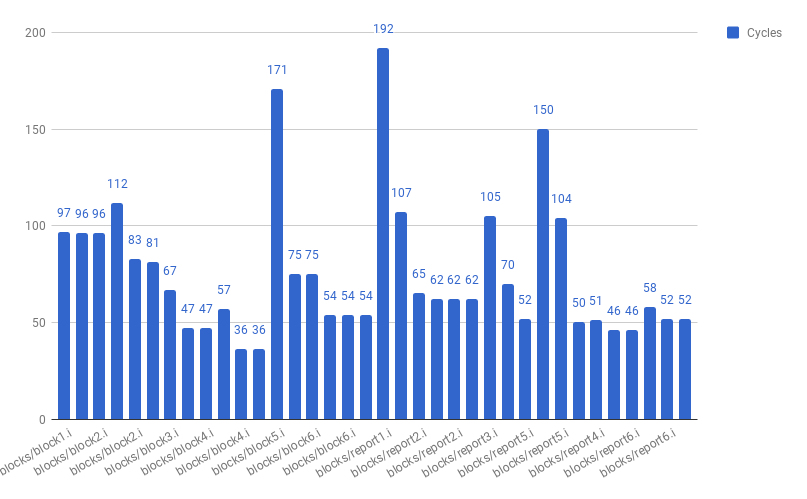
\includegraphics[scale=0.43]{b_cycles.png}
				\caption{In order, the number of cycles for the bottom-up allocator for 5, 10, and 20 registers for each of block1, block2, \dots, report 6. i.e: column 4 is 5 registers for block 2.}
			\end{figure}
	
			Observing the number of cycles required as the number of registers increase is unsurprising at first glance -- less registers are required to be spilled as $k$ increases. Since Bottom-Up allocators require no Feasible set $F$, all $k$ physical registers are able to be used throughout the allocated program. In blocks where MAXLIVE is $< k$, then, we find that the performance of the allocator is equivalent to the performance of the block without allocation, in terms of cycles. The upside of using the allocator, then, is the reduction in the number of registers: in \textit{block1}, for example, we can do with $k = 6$ registers and achieve the same number of cycles as the program written using $k = 50$ registers. 
			
			When $k = 5$, we experience the highest number of cycles compared to when $k = 10$ or $k = 20$, as previously discussed. The extent to which this difference occurs, though, can be dramatically altered by how often MAXLIVE $> k$. In \textit{block2}, \textit{report1}, and \textit{report5}, then, it makes sense that we see a dramatically higher number of cycles for $k = 5$ than when $k = 10$, since the number of instructions with MAXLIVE $> 5$ is larger than the number of instructions with MAXLIVE $> 10$. The number of instructions in which MAXLIVE exceeds $k$ is the biggest factor in how many extra registers need to be spilled. It makes sense, then, that in \textit{block1} we see such a small increase in the number of cycles required when $k = 5$ compared to when $k \geq 6$ -- only one instruction has a larger MAXLIVE than $5$, and so we only need to spill registers in that instruction. 
			
			This is a major upside when writing a compiler, so long as we assume that the values aren't intertwined too much. If users of the language are conscious of this and use variables that are not distributed throughout a block, the code produced can be very efficient even on machines with a low overall register count. This means that for Bottom-Up register allocators, it seems to be best to have many variables that are used quickly. Having variables that can be used once to perform a calculation and then used in the calculation following allows for an overall low MAXLIVE, but highly efficient register allocation scheme without much spilling, even when allowing hundreds of virtual registers.
			
			Another upside of the Bottom-Up allocator is that it runs linearly through the instruction block. That is, given $n$ instructions, it executes in $\Theta(n)$ time, as the allocator runs through each instruction, grabs a free register if available, or generates a spill instruction otherwise. The execution times in Figure 3, then, are all within negligibly close range to one-another. Running these tests several times yields execution times that show no significant statistical differences, since each testing block has roughly the same number of instructions.
			
		\begin{figure}[H]
			\centering
			\begin{tabular}{c|c|c|c|c}%
				 \bfseries File & \bfseries 5 Registers & \bfseries 10 Registers & \bfseries 20 Registers
				\csvreader[head to column names]{b_times.csv}{}% use head of csv as column names
				{\\\hline \file & \fiveregs & \tenregs & \twentyregs}
			\end{tabular}
			\caption{The execution times, in seconds, of the bottom up allocator for various $k$ values.}
		\end{figure}

	\subsection{Top Down EAC}
		\begin{figure}[H]
			\centering
			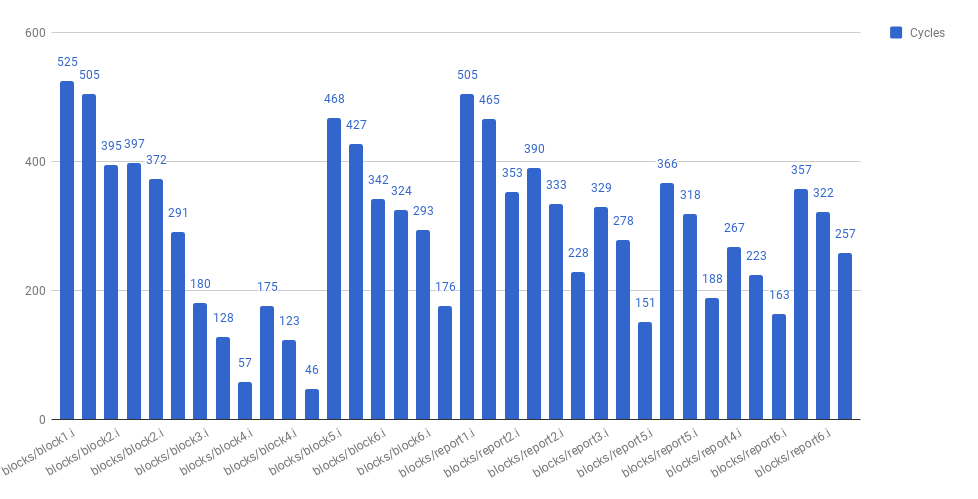
\includegraphics[scale=0.43]{s_cycles.png}
			\caption{In order, the number of cycles for the EAC top-down allocator for 5, 10, and 20 registers for each of block1, block2, \dots, report 6. i.e: column 4 is 5 registers for block 2.}
		\end{figure}
		
		The EAC version of the Top-Down allocator attempts to find the number of registers used least often throughout the block and use them as candidates for spillage. Unlike the Bottom-Up allocator, given $m$ registers in a block, this allocator will spill exactly $m - (k - F)$ registers, whereas the Bottom-Up allocator will spill only as needed. As such, when $k = 5$, this allocator must spill $50 - (5 - 2) = 47$ registers for \textit{block1}. Even when $k = 10$, it will need to spill $50 - 8 = 42$ registers, despite no instructions having a MAXLIVE $> 8$. 
		
		This allocator's largest downfall is in blocks which have registers heavily used in half of the block, but seldom used throughout, especially when many registers follow this pattern, as they all will be spilled. Register re-use could significantly make this a better algorithm, as we would not need to spill quite as many registers once they're no longer needed. That is, if a register is used to store $b = 2*a$, and then another register is used to store $b = 3*b$, we could reduce the number of registers needed by 1 by not using that second register. 
		
		In terms of execution times, this algorithm performed arguably the best, with the worst computation involved being a sort. Since in these test cases, the number of registers was fairly small, we utilized an insertion sort. Given $m$ registers and $n$ instructions, then, this entire algorithm ran in roughly $O(n + m^2)$. Since the number of registers is typically fairly small compared to the number of instructions in most of the blocks we tested, the entire algorithm runs in roughly $O(n)$, akin to the Bottom-Up allocator, but ran consistently faster than the other two allocators on all blocks. 
		
		\begin{figure}[H]
			\centering
			\begin{tabular}{c|c|c|c|c}%
				 \bfseries File & \bfseries 5 Registers & \bfseries 10 Registers & \bfseries 20 Registers
				\csvreader[head to column names]{s_times.csv}{}% use head of csv as column names
				{\\\hline \file & \fiveregs & \tenregs & \twentyregs}
			\end{tabular}
			\caption{The execution times, in seconds, of the EAC Top-Down allocator for various $k$ values.}
		\end{figure}

	\subsection{Top Down Class}
		\begin{figure}[H]
			\centering
			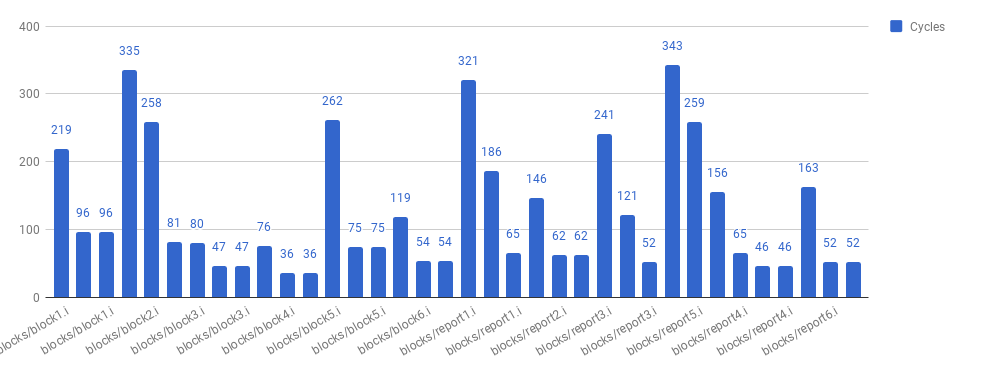
\includegraphics[scale=0.43]{t_cycles.png}
			\caption{In order, the number of cycles for the In-Class top-down allocator for 5, 10, and 20 registers for each of block1, block2, \dots, report 6. i.e: column 4 is 5 registers for block 2.}
		\end{figure}
		
		The In-Class Top-Down allocator is a major improvement over the EAC Top-Down allocator, given that it attempts to spill registers that actually are problematic in terms of the MAXLIVE with respect to $(k-F)$. Like the Bottom-Up compiler, there can be a reduction in the number of physical registers required to execute a block of instructions, without any increase in the number of cycles, so long as the MAXLIVE of every instruction is below a specific range. For this allocator, this occurs when the MAXLIVE of each instruction is $\leq (k - F)$. In \textit{block1}, for example, where the number of registers is 50, but MAXLIVE is $5$, we see nearly double the cycles required when $k = 5$ compared to the original block. When $k = 10$ (where $(10 - 2) \geq 5$) , however, the allocator is able to produce a block that takes exactly the same number of cycles as the original block, whereas the EAC Top-Down allocator required 505 cycles.
		
		These improvements aren't without cost. By far, this algorithm takes the longest to execute, as we must recompute the MAXLIVE of each instruction and continue through the process until all of the instructions are complete. It's difficult to bound exactly how many iterations much occur, as the number of instructions with MAXLIVE $> (k - F)$ can change depending on which register is spilled, but we can see from the run-time numbers that generally it performs significantly worse than the other allocators in wall-clock time.
		
		\begin{figure}[H]
			\centering
			\begin{tabular}{c|c|c|c|c}%
				 \bfseries File & \bfseries 5 Registers & \bfseries 10 Registers & \bfseries 20 Registers
				\csvreader[head to column names]{t_times.csv}{}% use head of csv as column names
				{\\\hline \file & \fiveregs & \tenregs & \twentyregs}
			\end{tabular}
			\caption{The execution times, in seconds, of the In-Class Top-Down allocator for various $k$ values.}
		\end{figure}
		
\section{Conclusion and Discussion}
	These allocators each have their strengths and weaknesses. For the EAC Top-Down Allocator, its biggest strength is its ease of implementation and quick runtime. There are very few obstacles in its implementation, as computing the number of occurrences can be done while interpreting each instruction. In that sense, the most difficult part of the algorithm is the sorting of the registers by the number of occurrences. That is about the extent of the successes for this particular allocator, though, as the number of cycles required to execute its code is always greater than the number of cycles in the block, so long as $(k+F) \leq $ MAXLIVE. In situations where the number of cycles aren't as significant as a quick implementation and a quickly running allocator, this is a great first stop. Register re-use also helps, as we can reduce the total number of registers used in the program.
	
	\begin{figure}[H]
			\centering
			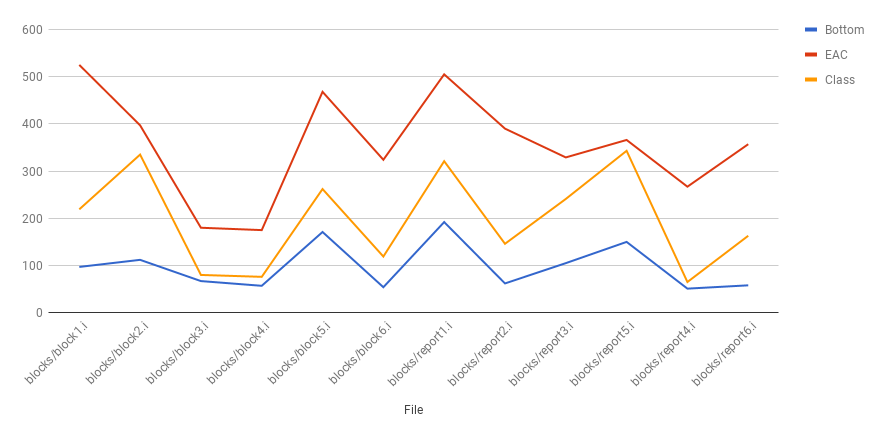
\includegraphics[scale=0.5]{all_cycles.png}
			\caption{Comparing the number of cycles required for each of the allocators one each block.}
		\end{figure}
	
	Between the Bottom-Up and In-Class Top-Down allocator, there are some trade-offs that need to be considered. In the implementation in our system, the In-Class Top-Down allocator was the most complex to implement, but that mostly was due to poor planning at the offset of the project. In terms of implementation difficulty with correct planning then, both algorithms seem equivalent in retrospect. When does one perform better than the other, then? Looking at the number of cycles, it seems that there was never a time in which the bottom-up allocator produced worse code than the other. The top-down allocator also took much longer to execute, and could potentially grow non-linearly as the MAXLIVE of each instruction grows, so it seems clear that the bottom-up allocator is the better choice in most cases.
	
	In personal testing, though, it seems that the Top-Down allocator used in class performed very well when the cause of instructions' MAXLIVE exceeding $(k - F)$ was due to several registers being used once in the beginning, not used during the duration of the program, and then used a final time at the very end of the program. In these situations, the allocator seemed to perform on-par with the Bottom-Up allocator (and in some cases even a bit better), while performing in nearly the same time complexity.
	
	What this essentially amounts to is understanding the typical code produced by the front-end of the compiler. If the ILOC code fed into the allocator is typically intertwined (and registers are used often) and performance of the final code matters, then it may be best to use the Bottom-Up allocator. In situations where registers are typically used once and then later on re-used towards the end of the block, and the running time of the allocator isn't as important, the In-Class Top-Down allocator seems fairly useful. When you just want to have something that runs really fast and isn't hard to implement correctly, or when register-reuse is allowed, the EAC version of the Top-Down allocator is a nice tool to have. Generally, the Bottom-Up allocator seemed to produced the best results, but these were just a few small testcases. Running these on blocks of thousands of instructions and with different characteristics throughout may shed light on different strategies that need to be utilized for the best results. 

\pagebreak

\begin{figure}[H]
			\centering
			\begin{tabular}{c|c|c|c|c}%
				 \bfseries Allocator & \bfseries File Name & \bfseries Number of Registers & \bfseries Cycles & \bfseries Execution Time
				\csvreader[head to column names]{all_cycles.csv}{}% use head of csv as column names
				{\\\hline \allocator & \file & \registers & \cycles & \time}
			\end{tabular}
			\caption{Full number of cycles and execution time for all allocators and report blocks for 5, 10, and 20 registers.}
		\end{figure}

\end{document}